%%%%%%%%%%%%%%%%%%%%%%%%%%%%%%%%%%%%%%%%%%%%%%%%%%%%%%%%%%%%%%%%%%%%%%
%%                     Association
%%%%%%%%%%%%%%%%%%%%%%%%%%%%%%%%%%%%%%%%%%%%%%%%%%%%%%%%%%%%%%%%%%%%%%

\subsection{Glyph: \glyph{Association}}\label{sec:association}

The association between one or more \glyph{EPNs} represents the non-covalent binding of the biological objects represented by those \glyph{EPNs} into a larger complex. An \glyph{association} between several entities is represented by a filled disc linked to two connectors separated by 180 degrees. The consumption (\sect{consumption}) and production (\sect{production}) arcs are linked to the extremities of those connectors. An \glyph{association} is never reversible, the inverse process being represented by a \glyph{dissociation} (\sect{dissociation}).

\begin{figure}[H]
  \centering
  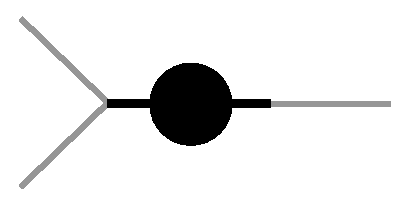
\includegraphics[scale = 0.5]{images/association}
  \caption{The \PD glyph for \glyph{association}.}
  \label{fig:association}
\end{figure}

The example in \fig{assoc-cyclin} illustrates the association of cyclin and CDC2 kinase into the Maturation Promoting Factor.

\begin{figure}[H]
  \centering
  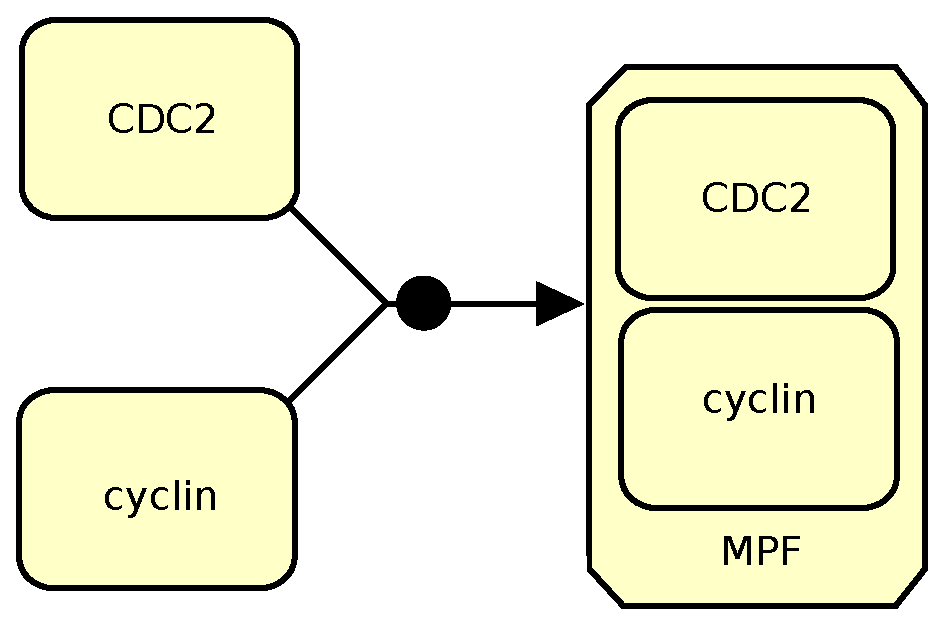
\includegraphics[scale = 0.5]{images/association-MPF}
  \caption{Association of cyclin and CDC2 kinase into the Maturation Promoting Factor.}
  \label{fig:assoc-cyclin}
\end{figure}

An \glyph{association} does not necessarily involve components of the same nature. \fig{assoc-unamed} gives an example illustrating the association of a pentameric \glyph{macromolecule} (a nicotinic acetylcholine receptor) with a \glyph{simple chemical} (the local anesthetic chlorpromazin) in an unnamed complex.

\begin{figure}[H]
  \centering
  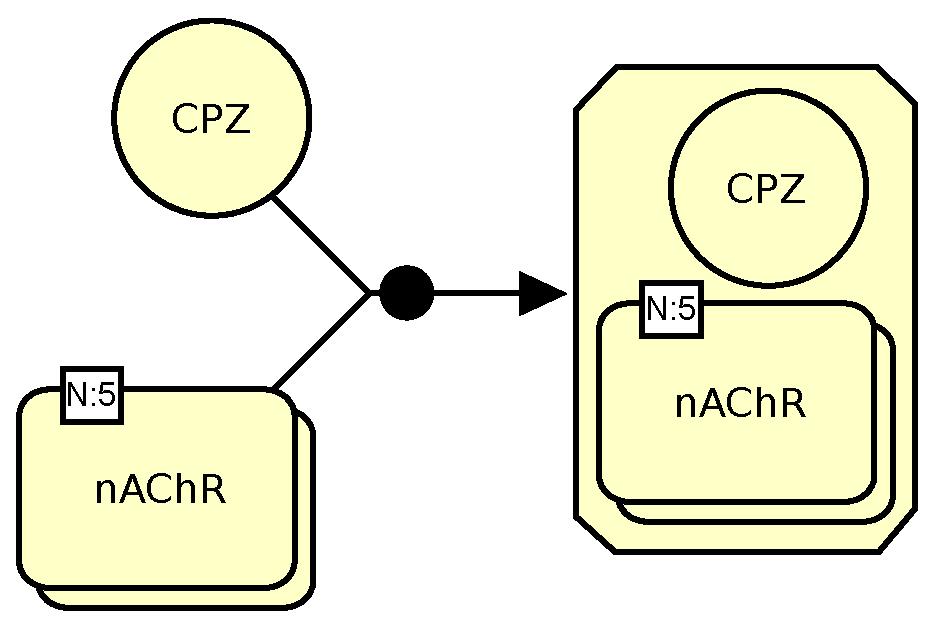
\includegraphics[scale = 0.5]{images/association-unamed}
  \caption{The association of a pentameric macromolecule with a simple chemical in an unnamed complex.}
  \label{fig:assoc-unamed}
\end{figure}

An association does not necessarily result in the formation of a \glyph{complex}; it can also produce a \glyph{multimer}. \fig{assoc-multi} gives an example of using the successive formation of an hemoglobin monomer then a tetramer of the resulting complex.

\begin{figure}[H]
  \centering
  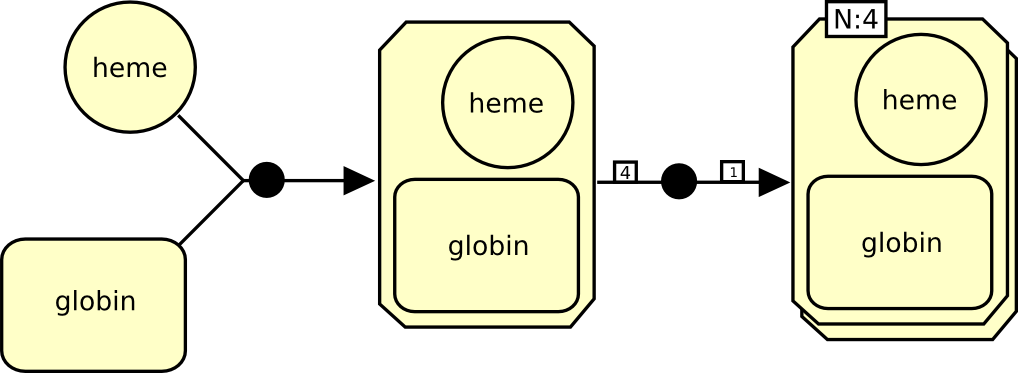
\includegraphics[scale = 0.5]{images/association-multimerisation}
  \caption{Formation of hemoglobin.}
  \label{fig:assoc-multi}
\end{figure}


